\documentclass{report}

\usepackage[italian]{babel}
\usepackage{graphicx}
\usepackage{hyperref}
\usepackage{listings}
\usepackage{xcolor}
\usepackage{tcolorbox}
\usepackage{etoolbox}
\usepackage{caption}
\usepackage{float}
\usepackage{listings}
\usepackage{needspace}

% Definizione di un nuovo ambiente per il rettangolo nero senza titolo (usato per mostrare i comandi da terminale)
\newtcolorbox{ret}{
    colback=white,
    colframe=black,
    boxrule=1pt,
    boxsep=5pt,
}

\newtcolorbox{warningbox}{
    colback=yellow!10, % Sfondo giallo chiaro
    colframe=yellow!80!black, % Bordo giallo scuro
    fonttitle=\bfseries, % Testo in grassetto
    title=Attenzione!, % Titolo del box
}

% Definisce il syntax highlighting per Groovy
\definecolor{groovyblue}{HTML}{0000A0}
\definecolor{groovygreen}{HTML}{008000}
\definecolor{darkgray}{rgb}{.4,.4,.4}

\lstdefinelanguage{Groovy}{
    keywordstyle=\color{groovyblue}\bfseries,
    stringstyle=\color{groovygreen}\ttfamily,
    keywords=[3]{each, findAll, groupBy, collect, inject, eachWithIndex},
    morekeywords={def, as, in, use},
    moredelim=[is][\textcolor{darkgray}]{\%\%}{\%\%},
    moredelim=[il][\textcolor{darkgray}]{§§}
}

% Disattiva lo spazio all'inizio delle nuove righe
\setlength{\parindent}{0pt}

\renewcommand{\thesection}{\arabic{section}} % Imposta la numerazione delle sezioni a partire da 1 invece che da 0 (1.n invece di 0.n.m)

\setcounter{tocdepth}{3} % Imposta la profondità dell'indice fino alle subsubsection

\begin{document}

    \begin{titlepage}
	\centering
    \graphicspath{{src/capitoli/01/img/}}
	
\includegraphics[width=0.7\textwidth, keepaspectratio]{logo-unitn.png}

	\vspace{1.3cm}
	\Large{Setup per il laboratorio di Programmazione 2\\}
	\vspace{0.4cm}
	\small{Come installare e configurare tutto il necessario per le lezioni di laboratorio}
\end{titlepage}

    \chapter*{Prefazione}
    In questa breve guida viene illustrato come installare e configurare tutto il necessario per poter seguire le lezioni di laboratorio.
    La guida si divide in due parti, la prima spiega cosa fare per poter svolgere gli esercizi usando il proprio computer, la seconda invece
    spiega come configurare IntelliJ sui computer di laboratorio per svolgere gli esercizi di JavaFx.\\
    La guida è svolta su Linux e Windows, se utilizzate un Mac, i passaggi sono pressochè gli stessi di Linux ma per quanto riguarda l'installazione
    di Java potete fare riferimento ai molti tutorial disponibili su internet.

    \begin{warningbox}
        Nessuno di questi passaggi sarà richiesto all'esame, vi verrà fornito IntelliJ IDEA con un template già configurato con tutto il necessario.
    \end{warningbox}
    
    \tableofcontents
    \section{Installare Java}

    In questo capitolo viene spiegato come installare Java, va bene una qualunque distribuzione (OpenJdk, Corretto etc...) e qualsiasi \textbf{versione maggiore o uguale alla 21}. Tenete a mente 
    che sui computer del laboratorio al momento della scrittura della guida è installata la vesione 21, perciò i comandi si riferiscono a quella versione.

    \subsection{Linux}
        Per installare Java su linux è sufficente utilizzare il gestore dei pacchetti della propria distribuzione, nel caso di\\
        \textbf{Debian, Ubuntu e derivate:}
        \begin{ret}
            \texttt{\$ sudo apt install openjdk-21-jdk -y}
        \end{ret}
        
        \textbf{Fedora, RHLE e derivate:}
        \begin{ret}
            \texttt{\$ sudo dnf install java-21-openjdk -y}
        \end{ret}

        \textbf{Arch e derivate:}
        \begin{ret}
            \texttt{\$ sudo pacman -S jdk21-openjdk}
        \end{ret}
        per tutte le altre distribuzione, vi invito a cercare su internet prestanto attenzione ad installare il \textbf{JDK} e non il JRE.
    
    \subsection{Windows}
        Su Windows useremo la distribuzione di Java di Amazon, chiamata Corretto, non ha nessuna differenza rispetto a OpenJdk, almeno per gli utilizzi che ne andremo a fare
        ma è più semplice da trovare e installare.

        per prima cosa scaricate l'installer \url{https://corretto.aws/downloads/latest/amazon-corretto-21-x64-windows-jdk.msi}\\
        nel caso in cui il link non sia più funzionante è sufficente cercare Corretto jdk 21, aprire la pagina di AWS e scaricare il file .msi per Windows x64.
    
    \subsection{MacOS}
    Su MacOS è importante fare attenzione a quale processore è presente nel vostro Mac
    \subsubsection{Chip M}
        Scaricate il file .pkg al seguente indirizzo \url{https://corretto.aws/downloads/latest/amazon-corretto-21-aarch64-macos-jdk.pkg} e installate il JDK.
    \subsubsection{Chip Intel}
        Scaricate il file .pkg al seguente link \url{https://corretto.aws/downloads/latest/amazon-corretto-21-x64-macos-jdk.pkg} e installate il JDK.
    
    \hfill \break
    Nel caso in cui il link per scaricare il pkg non sia più funzionante è sufficente cercare Corretto jdk 21, aprire la pagina di AWS e scaricare il file .pkg per MacOS prestando 
    attenzione all'architettura del vostro processore, se il vostro Mac ha un chip della \textbf{serie M} allora scaricate la versione \textbf{aarch64} se invece il vostro Mac
    ha un processore \textbf{Intel} scaricate la versione \textbf{x64}.
    \section{Installare IntelliJ}
    Per svolgere gli esercizi di laboratorio, le simulazioni e l'esame userete \textbf{IntelliJ IDEA Ultimate}, non è una scelta, perciò è utile che lo usiate anche 
    quando vi esercitate a casa, inoltre imparare le varie shortcuts da tastiera vi aiuterà molto durante l'esame, sopratutto quando dovrete fare dei refactors facendovi 
    risparmiare tempo prezioso.
    Il software è normalmente a pagamento ma gli studenti hanno diritto a una licenza gratuita annuale per tutti i prodotti JetBrains, il primo step è quindi ottenere la 
    certificazione di studente.
    \subsection{Registrarsi come studente}
        È possibile registrarsi in due modi, il primo consiste nell'usare l'indirizzo email di istituto ed è quello preferibile, mentre il secondo consiste nell'inviare il certificato
        di iscrizione in inglese.
        \begin{warningbox}
            Il secondo metodo è più lungo, richiede circa una settimana perché il certificato deve essere verificato da un essere umano, ma è talvolta necessario, nel caso 
            in cui il vostro indirizzo email non venga riconosciuto.
        \end{warningbox}
        Il mio consiglio è quello di provare a registrarvi con la mail e nel caso non venisse accettata, procedere con l'invio del certificato. Indipendentemente dal metodo scelto 
        recatevi al seguente link \url{https://www.jetbrains.com/shop/eform/students}
        
        \subsubsection{Email di istituto}
            Compilate il form, prestando attenzione ad inserire l'indirizzo email nel formato 
            \textbf{nome.cognome@studenti.unitn.it}.
            \begin{figure}[H]
                \centering
                \graphicspath{{src/capitoli/04/img/}}
                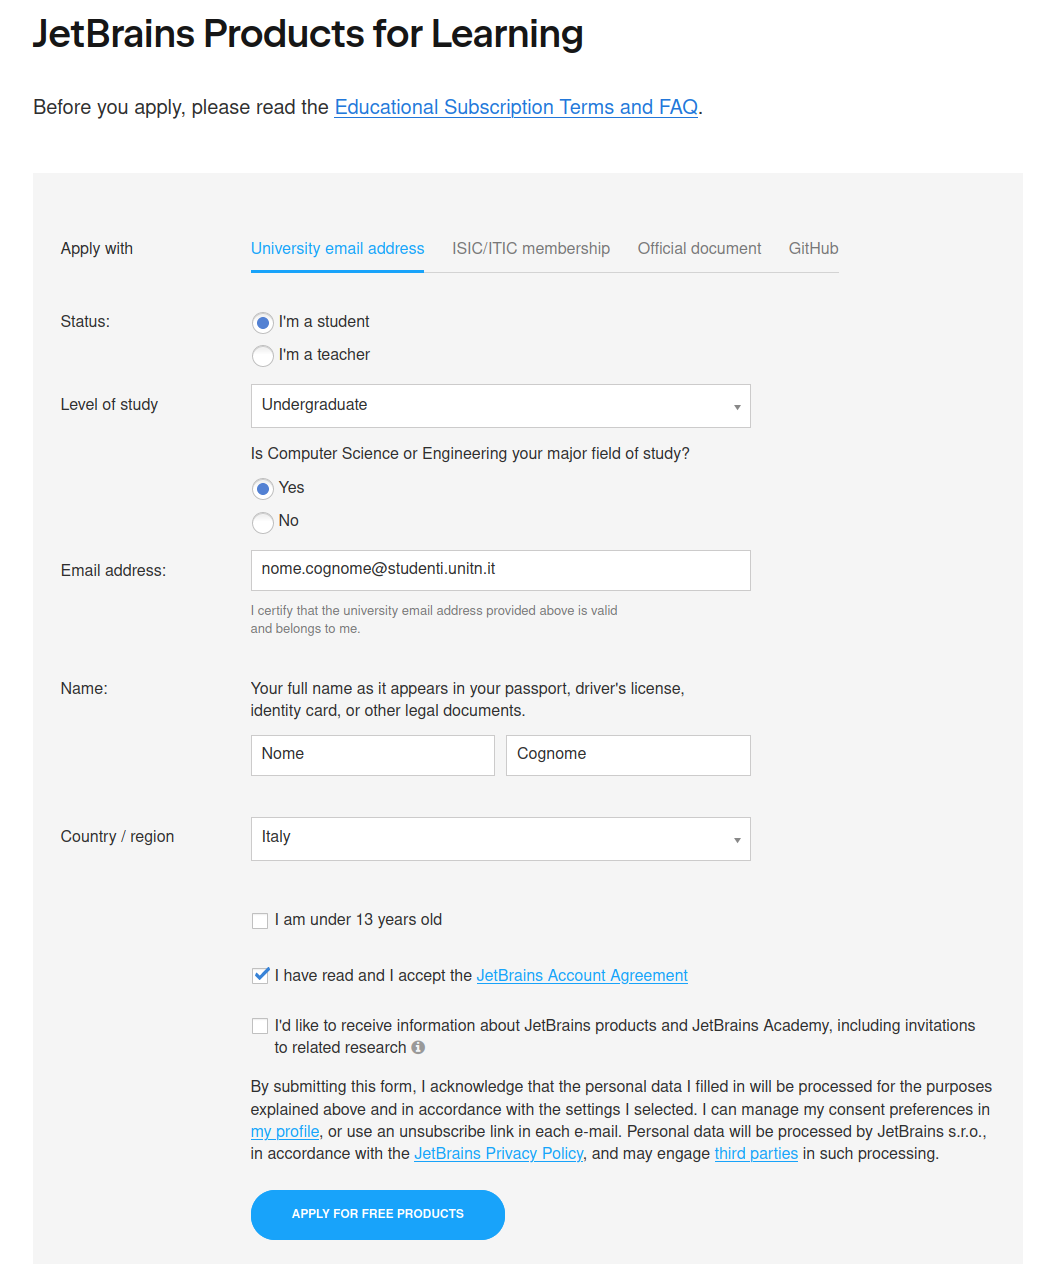
\includegraphics[width=1\textwidth]{form-studente-email.png}
                \caption{Form per la richiesta della licenza per studenti con email}
                \label{fig:Form per la richiesta della licenza per studenti con email}
            \end{figure}

            Una volta cliccato il bottone "Apply for free products" bisognerà completare il processo di certificazione aprendo il link ricevuto tramite email e completando 
            la creazione dell'account.
        
        \subsubsection{Certificato di iscrizione}
            Questa procedura richiede più passaggi, il primo dei quali è ottenere il certificato di iscrizione, andate su esse3, poi \textbf{Menù $\rightarrow$ Segreteria $\rightarrow$ My certificati} e in fine 
            cliccate su \textbf{Iscrizione con anni accademici (versione inglese)}. Scaricato il certificato tornate sulla pagina di JetBrains e selezionate apply with Official document, 
            compilate il form con i vostri dati, caricate il certificato e poi cliccate il bottone "Apply for free products".
            \begin{figure}[H]
                \centering
                \graphicspath{{src/capitoli/04/img/}}
                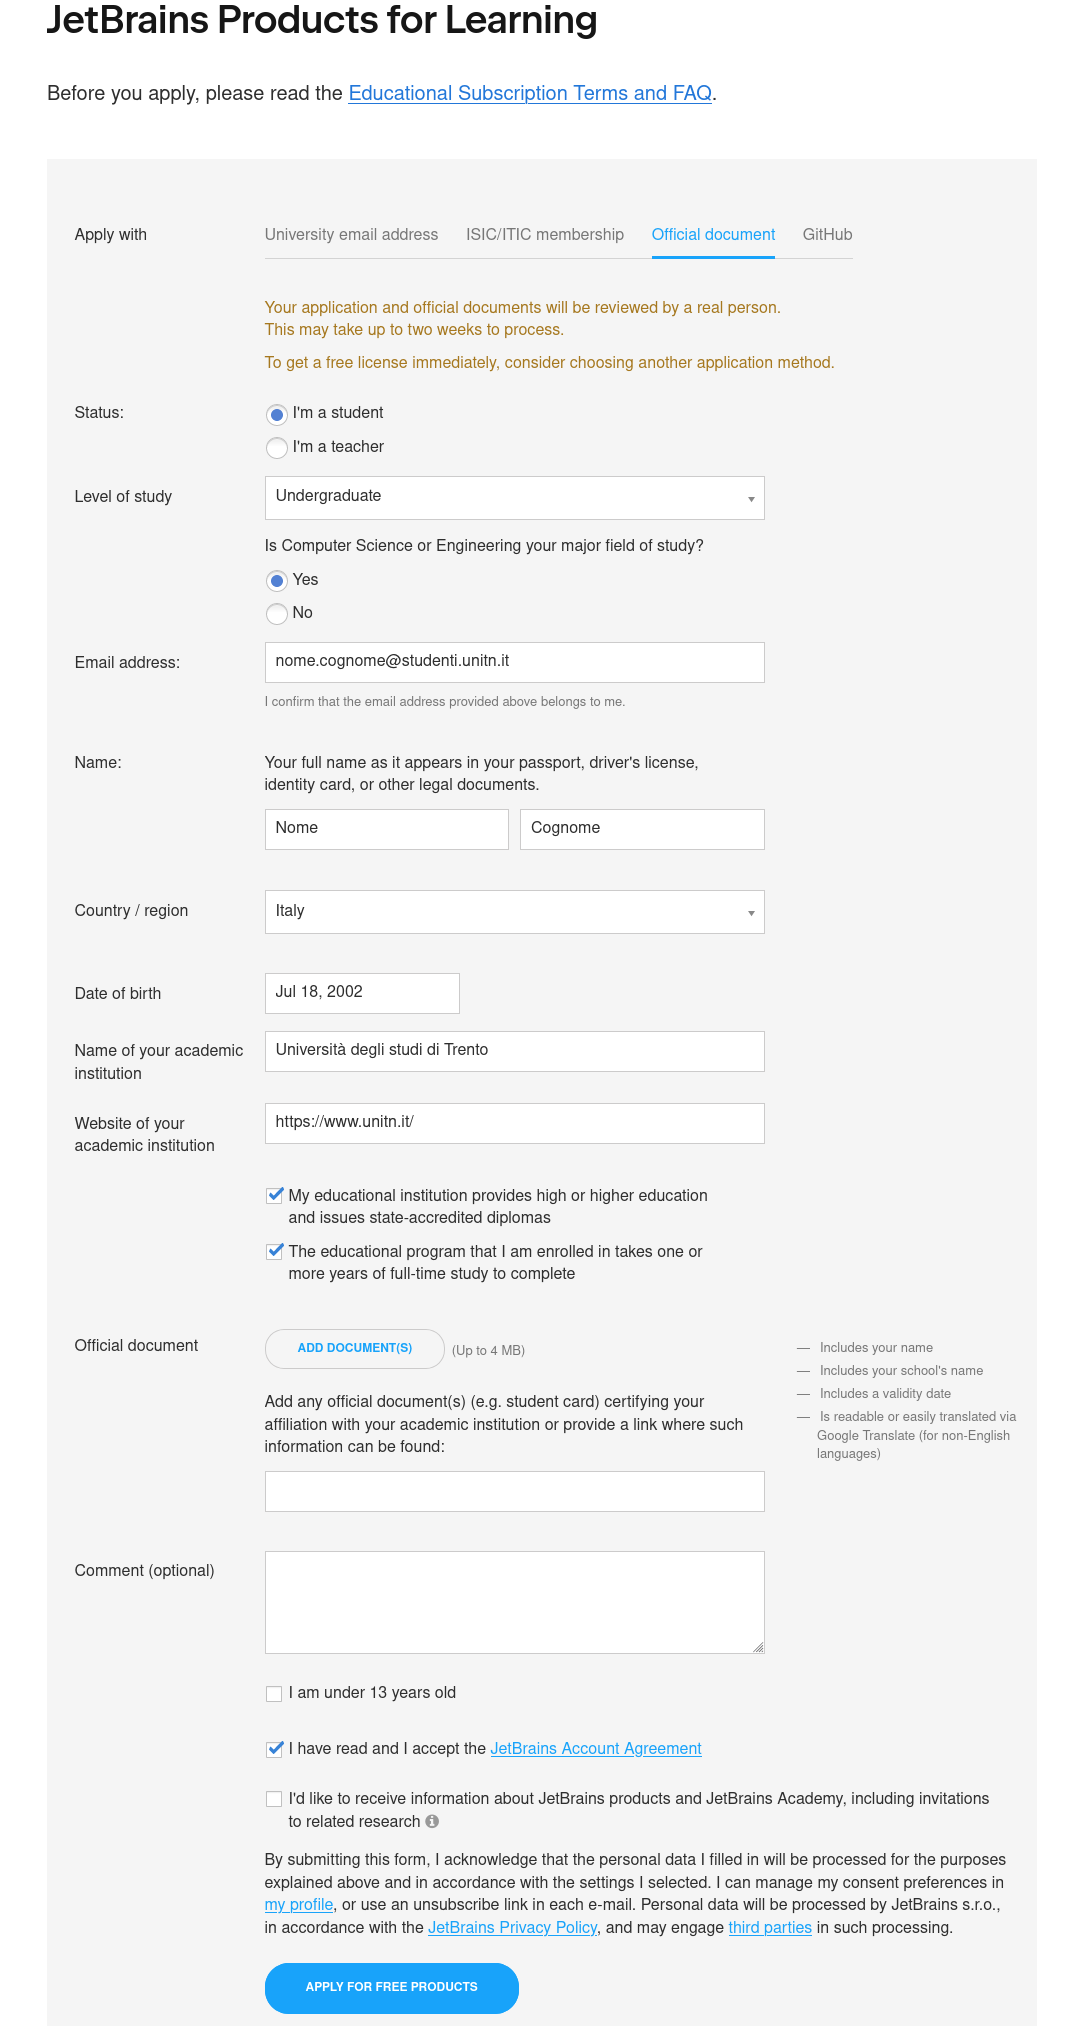
\includegraphics[width=0.7\textwidth]{form-studente-cert.png}
                \caption{Form per la richiesta della licenza per studenti con certificato}
                \label{fig:Form per la richiesta della licenza per studenti con certificato}
            \end{figure}
            Adesso dovete solo aspettare la mail di conferma per completare la creazione dell'account, solitamente richiede una settimana o più quindi abbiate pazienza.
    
    \subsection{Installare il ToolBox}
        Il modo più semplice per installare e mantenere aggiornati i prodotti JetBrains è utilizzare il ToolBox, un programma che consente di scaricare e mantenere aggiornati 
        tutti gli IDE di JetBrains, recatevi all'indirizzo \url{https://www.jetbrains.com/toolbox-app/}
        \subsubsection{Linux}
            scaricate il file .tar.gz, apritelo ed entrate nell'unica cartella presente, estraete il file e recatevi nella cartella in cui lo avete estratto. cliccate due volte col tasto 
            sinistro sul file chiamato jetbrains-toolbox e aspettate che vi si apra la seguente finestra (potrebbe richiedere qualche secondo)
            \begin{figure}[H]
                \centering
                \graphicspath{{src/capitoli/04/img/}}
                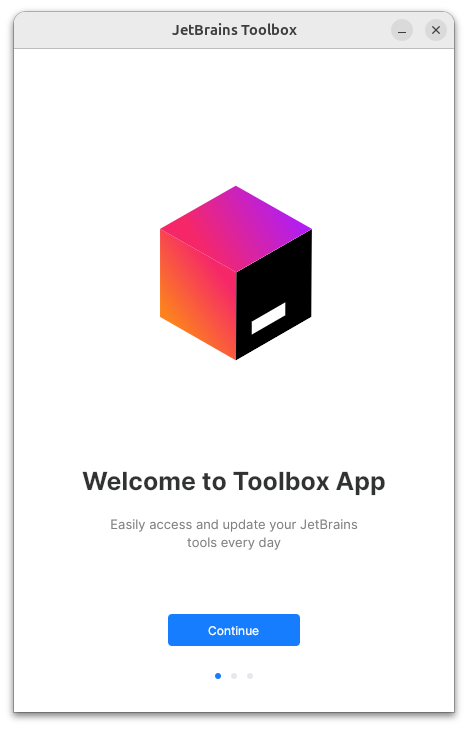
\includegraphics[width=0.5\textwidth]{toolbox-primo-avvio.png}
                \caption{Primo avvio del toolbox}
                \label{fig:Primo avvio del toolbox}
            \end{figure}
            cliccate su \textbf{Continue $\rightarrow$ Accept License Agreement $\rightarrow$ Get Started}.
            \begin{warningbox}
                Nel caso in cui la finestra non compaia (dopo aver aspettato un intervallo di tempo ragionevole), o l'abbiate chiusa per errore, 
                basterà andare nel \textbf{system tray} (barra delle notifiche), e cercare l'icona di una scatola rosa e nera. Per esempio in Ubuntu:
                \begin{figure}[H]
                    \centering
                    \graphicspath{{src/capitoli/04/img/}}
                    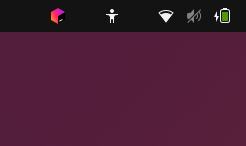
\includegraphics[width=0.5\textwidth]{barra-toolbox.png}
                    \caption{Icona del toolbox nel system tray di Gnome}
                    \label{fig:Icona del toolbox nel system tray di Gnome}
                \end{figure}
                se non fosse presente nel system tray, cercate nel menù delle applicazioni del vostro ambiente desktop, nel raro caso in cui non sia presente 
                nemmeno li, allora probabilmente vi manca \textbf{libfuse}, vi invito a \textbf{cercare su Google il nome della vostra distribuzione seguito dalla versione 
                e dalla frase "jetbrains toolbox won't start"}, sicuramente troverete una guida che saprà aiutarvi.
            \end{warningbox}
            A questo punto cliccate nella rotella in alto a destra e poi su \textbf{Log in}
            \begin{figure}[H]
                \centering
                \graphicspath{{src/capitoli/04/img/}}
                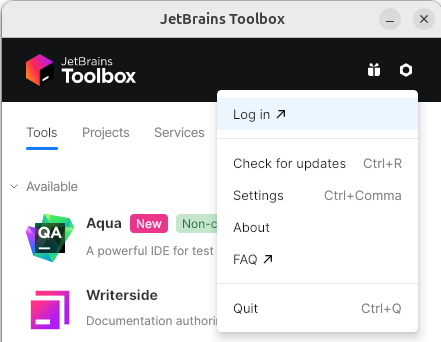
\includegraphics[width=0.35\textwidth]{toolbox-login.png}
                \caption{Menù per effettuare il login sul toolbox}
                \label{fig:Menù per effettuare il login sul toolbox}
            \end{figure}
    \section{Creare un progetto con JavaFx}
    Ora che avete tutto pronto, è im momento di creare un progetto con JavaFx, per farlo useremo Gradle, uno dei due build tool disponibili per Java.
    
    \subsection{Gradle}
        Un build tool è uno strumento che automatizza il processo di compilazione del codice sorgente, gestione delle dipendenze, esecuzione dei 
        test e creazione dei pacchetti eseguibili o distribuzioni del software. Una delle caratteristiche principali di Gradle è la 
        gestione delle dipendenze, che permette di dichiarare le dipendenze del progetto in modo semplice e le scarica automaticamente dai repository, 
        come pip per python o npm per node. Noi lo utilizzeremo proprio per gestire JavaFx, così da non dover scaricare a mano la libreria e la documentazione
        e cosa più importante non dovremo configurare a mano i moduli di JavaFx quando eseguiremo il progetto.

    \subsection{Nuovo progetto}
    Aprite IntelliJ e cliccate sul tasto \textbf{New Project}, come tipo di progetto scegliete Java, dategli il nome che preferite e salvatelo in una cartella a 
    vostra scelta.
    \begin{warningbox}
        Non scegliete come percorso per il progetto una chiavetta usb, sono memorie lente e questo renderebbe l'ide praticamente inutilizzabile.
        Imparate invece ad usare git.
    \end{warningbox}
    Importante è selezionare come \textbf{Build system Gradle}, e come \textbf{Gradle DSL Groovy}.Togliete pure la spunta su Add sample code.
    \begin{figure}[H]
        \centering
        \graphicspath{{src/capitoli/05/img/}}
        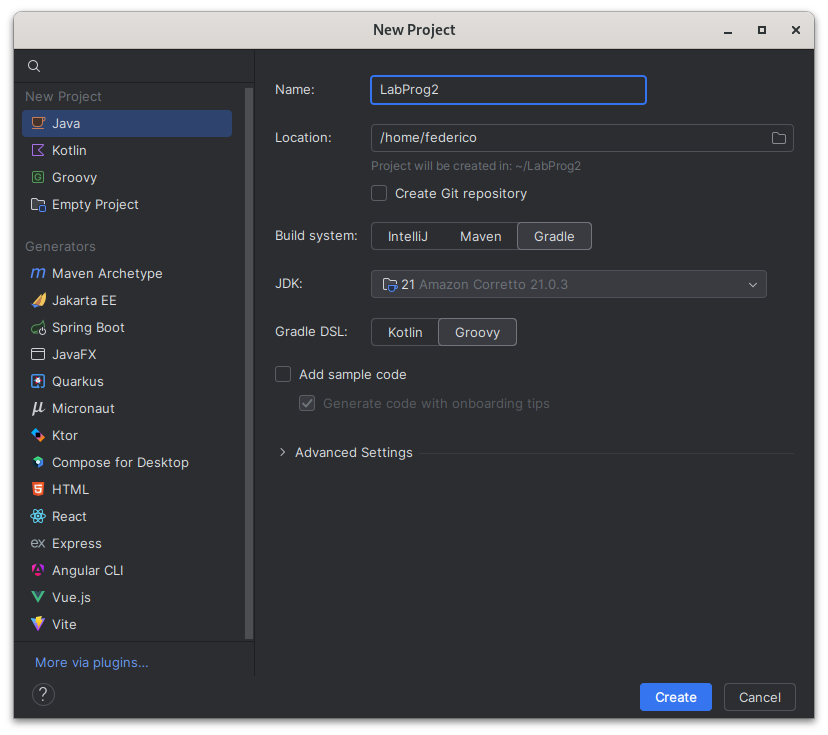
\includegraphics[width=\textwidth]{new_project.png}
        \caption{Creazione di un nuovo progetto con Gradle}
        \label{fig:Creazione di un nuovo progetto con Gradle}
    \end{figure}
    cliccate infine su Create e attendente la fine del processo.

    \subsection{Il file build.gradle}
    Una volta che il progetto sarà stato creato, vi si aprirà il file \textbf{build.gradle}, qui si specifica, tra le altre cose le dipendenze, 
    e come eseguire il vostro progetto. Se non vi si dovesse aprire in automatico, basta cercare il file nella barra laterale. Cancellate il 
    contenuto e incollate questo:
    \needspace{17\baselineskip}
    \begin{ret}
        \begin{lstlisting}[language=Groovy]
plugins {
    id 'application'
    id 'org.openjfx.javafxplugin' version '0.1.0'
}

group = 'org.example'
version = '1.0-SNAPSHOT'

repositories {
    mavenCentral()
}

javafx {
    version = "22" // versione di JavaFx
    modules = [ 'javafx.controls' ]
}

mainClassName = "Main"
        \end{lstlisting}
    \end{ret}
    \begin{warningbox}
        Controllate sul sito \url{https://gluonhq.com/products/javafx/} l'ultima versione di JavaFx compatibile con il vostro jdk.
    \end{warningbox}
    \begin{figure}[H]
        \centering
        \graphicspath{{src/capitoli/05/img/}}
        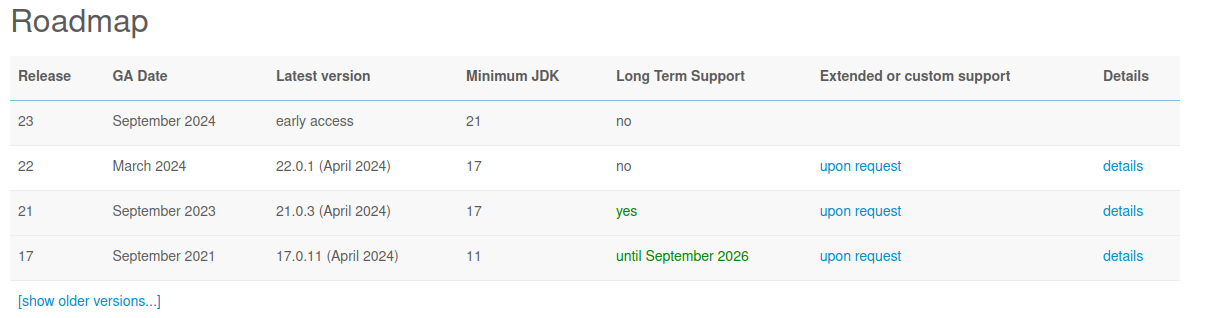
\includegraphics[width=\textwidth]{javafx_versions.png}
        \caption{Tabella con le versioni di JavaFx}
        \label{fig:Tabella con le versioni di JavaFx}
    \end{figure}    

    \subsection{Run configurations}
        Adesso che avete configurato Gradle per utilizzare JavaFx, cliccate in alto a destra il menù \textbf{Current File$\rightarrow$Edit Configurations$\rightarrow$+$\rightarrow$Gradle}
        \begin{figure}[H]
            \centering
            \graphicspath{{src/capitoli/05/img/}}
            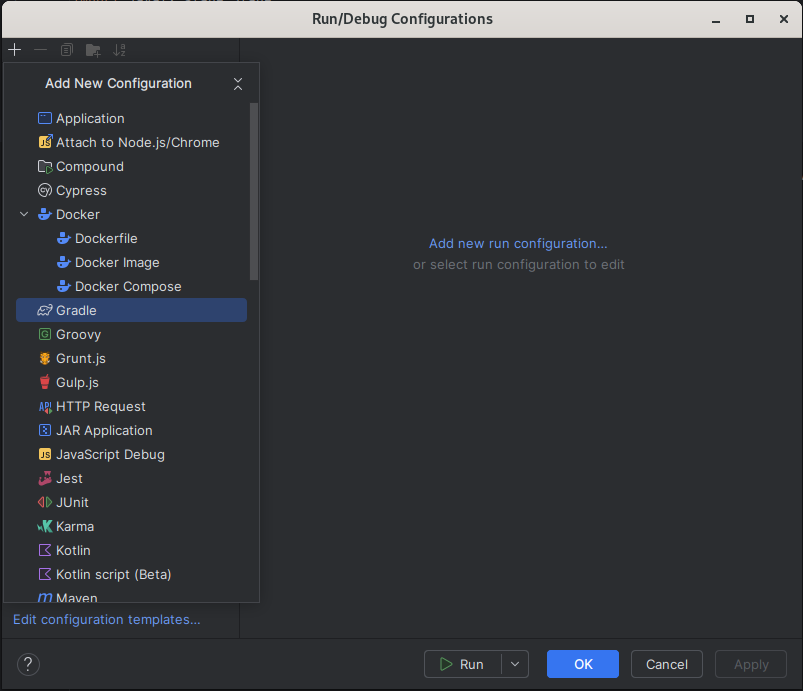
\includegraphics[width=\textwidth]{new_run_config.png}
            \caption{Menù opzioni di run}
            \label{fig:Menù opzioni di run}
        \end{figure}
        sotto \textbf{Run} nel campo di testo inserite il comando \texttt{run} questo specificherà che quando cliccherete il tasto esegui (quello a forma di 
        rettangolo verde) o il tasto di debug (quello a forma di insetto verde) eseguirà il comando run di Gradle caricando il modulo di JavaFx.
        L'opzione di run dovrebbe essere come questa:
        \begin{figure}[H]
            \centering
            \graphicspath{{src/capitoli/05/img/}}
            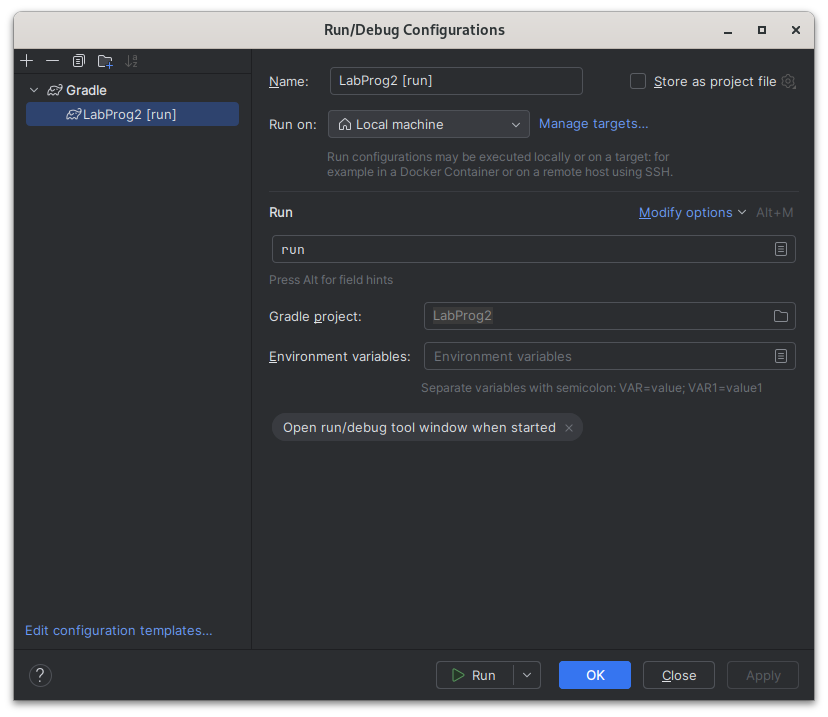
\includegraphics[width=\textwidth]{run_config.png}
            \caption{Opzione di run corretta per JavaFx}
            \label{fig:Opzione di run corretta per JavaFx}
        \end{figure}
    
    \subsection{Main di test}
        A questo punto per verificare che tutto sia correttamente configurato, aprite la cartella src, cancellate pure la sotto-cartella test e dentro la 
        sotto-cartella java create una nuova classe java chiamata Main. Cancellate tutto ciò che IntelliJ vi avrà creato e incollateci questo:
        \needspace{21\baselineskip}
        \begin{lstlisting}[language=Java]
import javafx.application.Application;
import javafx.scene.Scene;
import javafx.scene.control.Label;
import javafx.scene.layout.StackPane;
import javafx.stage.Stage;

public class Main extends Application {

    @Override
    public void start(Stage stage) {
        String javafxVersion = System.getProperty("javafx.version");
        Label l = new Label("Hello, JavaFX " + javafxVersion);
        Scene scene = new Scene(new StackPane(l), 640, 480);
        stage.setScene(scene);
        stage.show();
    }

    public static void main(String[] args) {
        launch();
    }
}            
        \end{lstlisting}
        Se tutto è configurato correttamente, cliccando il tasto di Run dovreste vedere una finestra come questa, con la versione di JavaFx che avete 
        specificato precedentemente.
        \begin{figure}[H]
            \centering
            \graphicspath{{src/capitoli/05/img/}}
            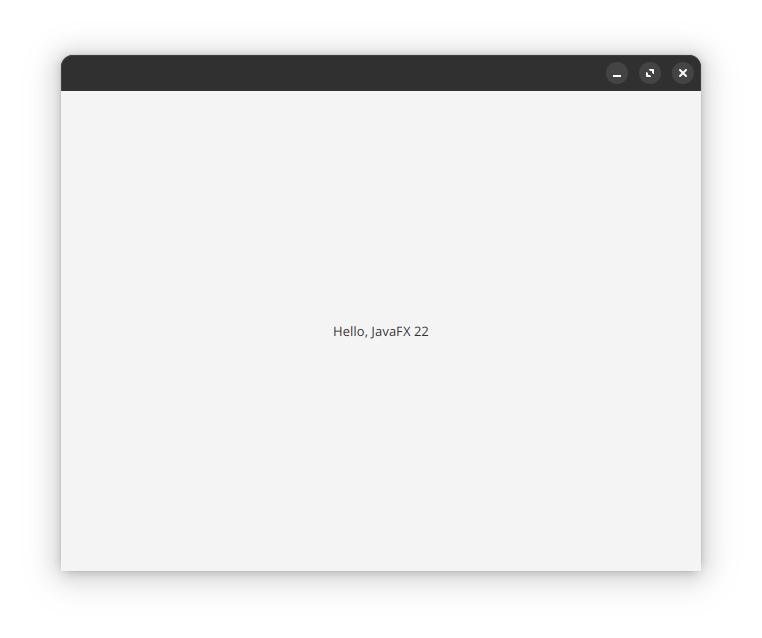
\includegraphics[width=\textwidth]{javafx_running.png}
            \caption{Finestra di prova}
            \label{fig:Finestra di prova}
        \end{figure}
        Non vi resta che seguire i vari laboratori, utilizzando la classe main che avete creato come base per completare le esercitazioni.

\end{document}